\chapter{Proof of Concept}
\label{ch:poc}

\section{Inleiding}

Dit hoofdstuk beschrijft de technische opzet en uitvoering van de Proof of Concept (PoC) ter validatie van het voorgestelde geïntegreerde framework. In het vorige hoofdstuk werd een risicoanalyse uitgevoerd die de kwetsbaarheden van AI-gedreven chatbots in kaart bracht, evenals de noodzaak om interacties traceerbaar te maken conform GDPR en enterprise-standaarden. Dit hoofdstuk vertaalt deze theoretische risicobeoordeling naar een concrete, technische implementatie.\\

De testomgeving bestaat uit een digitaal assistent-platform (Rasa) dat geïntegreerd is met een backend-architectuur. Eerst wordt de configuratie van de Akamai AI Firewall besproken, waarbij een onderscheid wordt gemaakt tussen vooraf gedefinieerde beveiligingsregels en applicatiespecifieke restricties. Vervolgens worden de toepassingsgebieden en de architecturale opzet van de chatbot toegelicht. Daarna wordt de geautomatiseerde testopstelling beschreven, waarmee kwaadaardige datastromen op een gecontroleerde manier worden gesimuleerd. Tot slot wordt de traceerbaarheid en observability binnen Dynatrace behandeld, inclusief het maskeren van gevoelige data en het correleren van incidenten.

\begin{figure}[H]
    \centering
    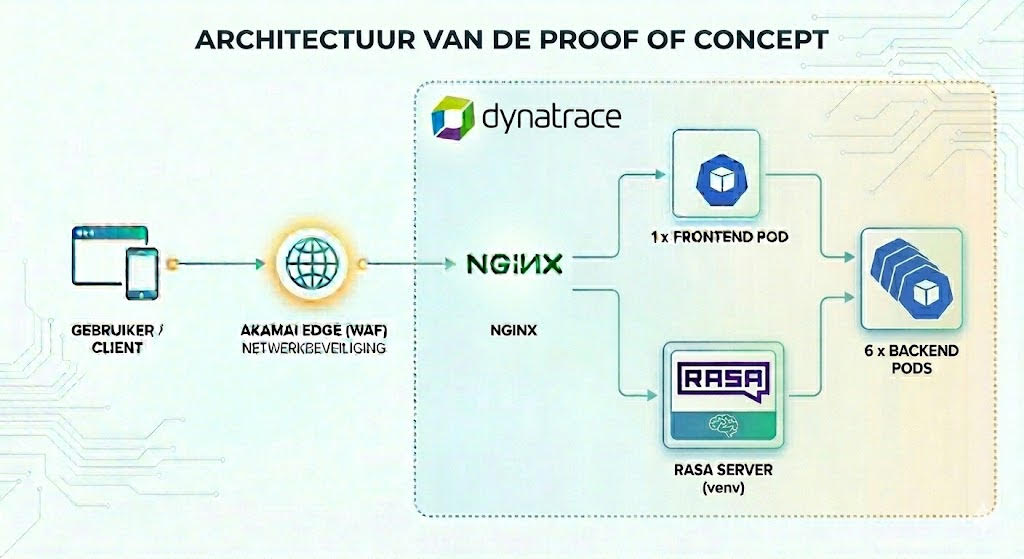
\includegraphics[width=0.75\textwidth]{img/opstelling.jpg}
    \caption{Opstelling PoC}
    \label{fig:gemini_architecture}
\end{figure}

\section{AI Firewall Regels en Configuratie}

Net zoals in traditionele beveiligingsoplossingen vormt de configuratie van de inspectieregels de kern van de applicatiebeveiliging. Binnen deze PoC fungeert de Akamai AI Firewall als de preventieve schil rond de chatbot. Omdat de communicatie tussen de frontend en de digitale assistent verloopt via een REST API met JSON-payloads, moeten de beveiligingsregels hierop worden afgestemd.

\subsection{Architecturale Context: Intent-gebaseerde NLU versus Generatieve AI}

Hoewel Akamai semantische inspectiemodules in de markt zet als specifieke bescherming voor Large Language Models (LLM's), is het essentieel om de architecturale context van deze PoC te benadrukken. De gebruikte digitale assistent (Rasa) is een intent-gebaseerd Natural Language Understanding (NLU)-systeem en geen generatief taalmodel. Hierdoor is de applicatie van nature immuun voor LLM-specifieke kwetsbaarheden zoals Prompt Injection of Jailbreaking; onverwachte of dwingende instructies resulteren simpelweg in een intent-fallback. Desondanks bewijst deze PoC dat de inzet van deze semantische AI-filters op de inkomende en uitgaande JSON-payloads enorme waarde biedt.

\subsection{Input Filtering (Bescherming van de backend)}

De eerste verdedigingslinie richt zich op het beveiligen van de inkomende gebruikersinvoer (input). Hierbij wordt de prompt van de gebruiker semantisch en syntactisch geanalyseerd voordat deze de applicatielaag (Rasa/Helidon) bereikt. In Tabel 5.1 worden de specifieke firewall-detectiemogelijkheden gekoppeld aan de geteste use-cases en dreigingen.

\begin{table}[H]
    \centering
    \caption{Mapping van Input Firewall-regels naar Use-Cases}
    \begin{tabular}{|p{4cm}|p{4cm}|p{6cm}|}
        \hline
        Akamai AI Capability & Use-Case & Toelichting \\
        \hline
        Code detected on input & XSS \& Injecties & Detecteert scripts zoals \texttt{<script>alert(1)</script>} \\
        \hline
        Input too long & DoS \& Overflow & Beperkt payload lengte \\
        \hline
        PII input & GDPR \& PCI-DSS & Detecteert gevoelige input \\
        \hline
        Toxic input & Abuse filtering & Blokkeert ongepast gedrag \\
        \hline
        Non-allowed language & WAF evasion & Blokkeert vreemde talen \\
        \hline
    \end{tabular}
\end{table}

\subsection{Output Filtering (Bescherming van de eindgebruiker en bedrijfsdata)}

Hoewel het systeem geen probabilistische teksten genereert, volstaat het niet om enkel de invoer te controleren. De backend-database kan reeds gecompromitteerd zijn, of de bedrijfslogica kan onverwacht reageren op een query (bijvoorbeeld door te veel data op te halen). Daarom implementeert de PoC tevens output filtering, waarbij het antwoord van de chatbot wordt geïnspecteerd voordat het over het netwerk naar de eindgebruiker wordt teruggestuurd.

\begin{table}[H]
    \centering
    \caption{Mapping van Output Firewall-regels}
    \begin{tabular}{|p{4cm}|p{4cm}|p{6cm}|}
        \hline
        Akamai AI Capability & Use-case & Toelichting \\
        \hline
        PII output & IDOR & Detecteert gevoelige output \\
        \hline
        Output too long & Data dumping & Voorkomt massale responses \\
        \hline
        Code detected on ouput & XSS & Blokkeert scripts \\
        \hline
        Toxic output & Echo prevention & Blokkeert toxische output \\
        \hline
    \end{tabular}
\end{table}

\section{Systeemarchitectuur en Integratie}

De architectuur van deze Proof of Concept is ontworpen als een hybride omgeving. Dit houdt in dat de webinterface en de backend-logica draaien binnen geïsoleerde Docker-containers (pods), terwijl de chatbot (Rasa) direct op de server draait in een lokale Python-omgeving (venv). Om dit netwerkverkeer veilig en gestructureerd te routeren, volgt de datastroom een strikt pad. Een verzoek van de eindgebruiker passeert allereerst de Akamai Edge firewall ter inspectie. Daarna komt het gezuiverde verkeer aan op de on-premise host, waar Nginx dient als de centrale verkeersregelaar. Nginx verdeelt deze inkomende verzoeken vervolgens over de juiste Docker-pods en de lokale virtuele omgeving.

\subsection{Hybride Infrastructuur: Kubernetes-omgeving en Virtual Environments}

Voor de uitvoering van de Proof of Concept is gekozen voor een architectuur die schaalbaarheid combineert met isolatie. De ondersteunende infrastructuur is ondergebracht in een Kubernetes-cluster, waarbij de verschillende componenten draaien als Pods. De kern van de digitale assistent draait daarentegen in een specifieke Python-omgeving op de host-machine. Deze hybride opzet bestaat uit de volgende technische componenten:

\begin{itemize}
    \item \textbf{Frontend-pod}: Een gecontaineriseerde web-widget die de gebruikersinterface ontsluit en de communicatie met de API verzorgt via een Kubernetes Service.
    \item \textbf{Rasa NLU (Local venv)}: De digitale assistent draait binnen een Python Virtual Environment (venv) op de host-node. Dit stelt de assistent in staat om direct gebruik te maken van de systeembronnen voor intent-extractie en dialoogbeheer zonder de netwerk-overhead van een extra containerlaag binnen het cluster.
    \item \textbf{Backend-pods (Java/Helidon)}: Zes gecontaineriseerde microservices die binnen het Kubernetes-cluster de bedrijfslogica en productgegevens van de 'Sockshop' beheren.
\end{itemize}

In Listing~\ref{lst:front-end} is de definitie van de frontend-laag weergegeven middels een Kubernetes manifest. Hierin is te zien hoe de frontend als een Deployment en Service wordt gedefinieerd, waarbij Rasa bewust buiten deze omgeving is gelaten.

\begin{lstlisting}[language={}, caption={Kubernetes manifest voor de frontend-laag met custom web-widget}, label={lst:front-end}, breaklines=true, numbers=left,frame=single]
kind: Service
apiVersion: v1
metadata:
  name: front-end
  labels:
    app: front-end
spec:
  type: ClusterIP
  ports:
  - port: 80
    targetPort: 8079
  selector:
    app: front-end
---
kind: Deployment
apiVersion: apps/v1
metadata:
  name: front-end
spec:
  replicas: 1
  selector:
    matchLabels:
      app: front-end
  template:
    metadata:
      labels:
        app: front-end
    spec:
      nodeSelector:
        beta.kubernetes.io/os: linux
      containers:
      - name: front-end
        image: my-custom-frontend:v1
        imagePullPolicy: Never
        env:
        - name: DT_SUPPORT_DEPRECATED_NODE_VERSIONS
          value: "true"
        - name: CARTS_HOST
          value: "carts"
        - name: CARTS_PORT
          value: "80"
        resources:
          requests:
            cpu: 100m
            memory: 200Mi
          limits:
            cpu: 1000m
            memory: 200Mi
        ports:
        - containerPort: 8079
        securityContext:
          runAsNonRoot: true
          runAsUser: 10001
            capabilities:
              drop:
                - all
            readOnlyRootFilesystem: true
\end{lstlisting}

\subsection{Rasa NLU \& Custom REST Channel Configuratie}

Zoals eerder De configuratie van de digitale assistent vormt een cruciaal onderdeel van de beveiligingsketen. In de standaardconfiguratie maakt Rasa vaak gebruik van WebSockets (via Socket.IO) voor real-time communicatie. Tijdens de initiële integratietests werd echter vastgesteld dat de specifieke protocol-framing van Socket.IO (bijvoorbeeld de numerieke 42 prefix voor berichten) de JSON-structuur 'vervuilt'. Dit maakte het voor de Akamai Firewall for AI onmogelijk om de payload semantisch te parsen en de geconfigureerde JSONPath-inspectie op het \texttt{\$.message} veld toe te passen.\\

Om deze beperking te omzeilen, is er een architecturale keuze gemaakt voor een Custom REST Channel. De frontend is zodanig geherprogrammeerd dat chatberichten als zuivere HTTP POST-requests worden verzonden. In de credentials.yml van Rasa is hiervoor het rest kanaal geactiveerd. Deze aanpassing garandeert dat de data die de Firewall for AI passeert een valide JSON-object is, zoals weergegeven in Listing~\ref{lst:rasa_json}. Hierdoor kan de firewall de inspectieregels voor XSS, SQLi en PII-detectie met maximale precisie uitvoeren op de werkelijke inhoud van het bericht.

\begin{lstlisting}[language={}, caption={Structuur van de REST-payload voor optimale WAF-inspectie}, label={lst:rasa_json}, breaklines=true, numbers=left,frame=single]
    {        
        "sender": "gebruiker_123", 
        "message": “Waar kan deze chatbot me mee helpen?” 
    }
\end{lstlisting}

\subsection{Nginx Gateway en Routing}

De Nginx-container dient als de kritieke schakel in de architectuur. Het vormt niet alleen de verbinding met de Akamai Firewall, maar verzorgt ook de routing tussen de verschillende werkomgevingen (pod naar venv). De configuratie is zodanig opgesteld dat inkomend verkeer van de Firewall wordt gedistribueerd naar de juiste laag.\\

In de onderstaande configuratie is te zien hoe Nginx verzoeken doorstuurt naar de Rasa-service die buiten Docker draait, door gebruik te maken van\\ \texttt{http://localhost:5005/webhooks/secure\_rest/}.

\begin{lstlisting}[language={bash}, caption={Nginx configuratie fragment voor routing tussen pods en venv}, label={lst:nginx}, breaklines=true, numbers=left,frame=single]
location /webhooks/secure_rest/ {    
  proxy_pass http://localhost:5005/webhooks/secure_rest/;    
  proxy_set_header Host $host;    
  proxy_set_header X-Real-IP $remote_addr;   
  proxy_set_header X-Forwarded-For $proxy_add_x_forwarded_for;    
  proxy_set_header X-Forwarded-Proto $scheme;    
  proxy_hide_header 'Content-Type';    
  add_header 'Content-Type' 'application/json' always;    
}
\end{lstlisting}

Deze hybride opzet garandeert dat de Akamai AI Firewall volledige zichtbaarheid heeft over het HTTP/REST-verkeer voordat het de host bereikt. Tegelijkertijd zorgt de installatie van de Dynatrace OneAgent op het besturingssysteem (systemctl) ervoor dat zowel de lokale Python-processen in de venv als de containers in de Docker-runtime binnen dezelfde trace worden gevangen.

\subsection{Geautomatiseerde Opstart van de Testomgeving}

Omdat de hybride testomgeving bestaat uit meerdere losse componenten—een Kubernetes-cluster met microservices en een lokale Python-omgeving voor de chatbot—vereist het handmatig opstarten veel herhalend typewerk. Om de omgeving voor elke test snel en in een consistente staat op te leveren, is een praktisch Bash-script geschreven.\\

Dit opstartscript \texttt{(start\_dev.sh)} automatiseert de volgende dagelijkse acties:

\begin{itemize}
    \item \textbf{Netwerktoegang (Port-Forwarding)}: Het legt verbindingen (kubectl port-forward) naar de afzonderlijke Kubernetes-services (zoals de frontend, catalogus en user-API's), zodat deze microservices bereikbaar worden op localhost.
    \item \textbf{Rasa Initialisatie}: Het activeert de lokale Python virtual environment (venv) en start zowel de Rasa NLU-engine als de bijbehorende action server op in de achtergrond.
    \item \textbf{Schoon Afsluiten (Graceful Shutdown)}: Dankzij een trap-functie in Bash worden al deze achtergrondprocessen aan het eind van een test netjes in één keer afgesloten zodra de gebruiker Ctrl+C indrukt.
\end{itemize}

\begin{lstlisting}[language={bash}, caption={Bash-script voor het efficiënt opstarten en afsluiten van de hybride PoC-omgeving}, label={lst:opstartscript}, breaklines=true, numbers=left,frame=single]
#!/bin/bash

echo "🚀 Starting Sock Shop & Rasa Dev Environment..."

# This 'trap' catches Ctrl+C and kills all the background processes cleanly
cleanup() {  
    echo ""    
    echo "🛑 Shutting down all services..."    
    kill $(jobs -p)    
    echo "✅ All services stopped."    
    exit
    }

trap cleanup SIGINT SIGTERM

# 1. Start Frontend Port Forward (External access for Webshop)
echo "➡️ Starting Frontend Port-Forward (Port 8079)..."
kubectl port-forward --address 127.0.0.1 svc/front-end 8079:80 -n sockshop-core > frontend_pf.log 2>&1 &

echo "Starting Sock Shop API Port-Forwards..."

# 1. Catalogue API (For getting item names/details)
kubectl port-forward svc/catalogue 8081:80 -n sockshop-core > /dev/null 2>&1 &

# 2. Carts API (For managing the shopping cart)
kubectl port-forward svc/carts 8082:80 -n sockshop-core > /dev/null 2>&1 &

# 3. User API (For translating IDs and getting profiles)
kubectl port-forward svc/user 8083:80 -n sockshop-core > /dev/null 2>&1 &

# 4. Orders API (For checking out and order history)
kubectl port-forward svc/orders 8084:80 -n sockshop-core > /dev/null 2>&1 &

# 5. Shipping API (HTTP REST endpoint)
kubectl port-forward svc/shipping-http 8085:80 -n sockshop-core > /dev/null 2>&1 &

# 6. Payment API (HTTP REST endpoint)
kubectl port-forward svc/payment-http 8086:80 -n sockshop-core > /dev/null 2>&1 &

# === THE FIX: Move into the correct directory ===
echo "➡️ Moving to Rasa project folder..."
cd ~/rasa-ecommerce

# Activate Virtual Environment for Rasa
echo "➡️ Activating Python virtual environment..."
source venv/bin/activate

# 3. Start Rasa Action Server
echo "➡️ Starting Rasa Action Server (Port 5055)..."
rasa run actions > action_server.log 2>&1 &

# 4. Start Rasa Main Server
echo "➡️ Starting Rasa Main Server (Port 5005)..."
rasa run --enable-api --cors "*" --port 5005 > rasa_server.log 2>&1 &

echo ""
echo "🎉 All systems go! Services are booting up in the background."
echo "You can view the logs in real-time by running 'tail -f [log_name]'"
echo "⚠️  Press Ctrl+C to stop all services and exit."

# This command keeps the script open so the background jobs stay alive
wait  add_header 'Content-Type' 'application/json' always;    
    }
\end{lstlisting}


\subsection{Interne Configuratie en Logica van de Digitale Assistent}

In tegenstelling tot generatieve taalmodellen (LLM's) die autonoom antwoorden formuleren, werkt deze chatbot op basis van een deterministische, intent-gedreven pijplijn. De configuratie is opgedeeld in drie kerncomponenten:\\

\begin{enumerate}
    \item \textbf{Natural Language Understanding (NLU)} Inkomende tekst van de gebruiker wordt door de NLU-engine verwerkt aan de hand van de trainingsdata in het nlu.yml bestand. De engine heeft twee doelen: het classificeren van de intentie van de gebruiker (de intent, bijvoorbeeld \texttt{check\_cart}) en het extraheren van specifieke parameters (de entities, zoals een tag of \texttt{user\_id}).
    \item \textbf{Dialogue Management (Core)} De reactie van de chatbot op een specifieke intent is vastgelegd in de stories.yml en rules.yml bestanden. Deze bestanden definiëren de gespreksflow. Wanneer het systeem bijvoorbeeld de intentie \texttt{get\_order\_status} herkent, dicteert een rule dat de assistent een geprogrammeerde actie moet uitvoeren, in plaats van simpelweg een statisch tekstbericht terug te sturen.
    \item \textbf{De Action Server (Backend Integratie)} Dit is vanuit beveiligingsperspectief het meest kritieke onderdeel van de architectuur. De Custom Actions (geschreven in Python binnen het actions.py bestand) vormen de brug tussen de NLP-engine en de Kubernetes-infrastructuur. Wanneer een actie wordt getriggerd, voert de Action Server een API-call uit naar de interne Helidon microservices (zoals weergegeven in de port-forwards van het opstartscript).
\end{enumerate}

\begin{lstlisting}[language={python}, caption={fragment van een Custom Action die de backend aanspreekt}, label={lst:checkCart}, breaklines=true, numbers=left,frame=single]
class ActionCheckCart(Action):
    def name(self) -> str:
        return "action_check_cart"

    def run(self, dispatcher: CollectingDispatcher,
        tracker: Tracker,
        domain: Dict[Text, Any]) -> List[Dict[Text, Any]]:

        with tracer.start_as_current_span("CheckCart"):
        # 1. Check the Rasa Slot first (this is where it should be stored)
        target_id = tracker.get_slot("username")
        print(tracker.latest_message)
        # 2. Fallback to metadata just in case it's the very first message
        if not target_id:
            metadata = tracker.latest_message.get("metadata", {})
            target_id = metadata.get("username", "guest")

        print(f"--- FETCHING CART FOR: {target_id} ---")

        try:
            res = requests.get(f"http://127.0.0.1:8082/carts/{target_id}/items", timeout=2)
            if res.status_code == 200:
                items = res.json()
                if items and len(items) > 0:
                    response = f"I found {len(items)} item(s) in your cart:\n"
                    for i in items:
                        name = i.get("itemId")
                        try:
                            cat = requests.get(f"http://127.0.0.1:8081/catalogue/{name}", timeout=1).json()
                            name = cat.get("name", name)
                        except:
                            pass
                        response += f"* {i.get('quantity')}x **{name}**\n"
                    dispatcher.utter_message(text=response)
                else:
                    dispatcher.utter_message(text=f"Your cart is empty. (User: {target_id})")
                else:
                    dispatcher.utter_message(text="I can't reach your cart right now.")
            except Exception as e:
                print(f"Error fetching cart: {e}")
                dispatcher.utter_message(text="Warehouse connection error.")

            return []
\end{lstlisting}


\section{Dynatrace Observability en Traceerbaarheid}

Waar de Akamai firewall dient als het preventieve schild aan de rand van het netwerk, levert Dynatrace de audit trail en end-to-end zichtbaarheid binnen de applicatie-infrastructuur. Het doel van deze integratie is niet alleen het monitoren van prestaties en foutcodes, maar het creëren van een sluitend, juridisch en technisch verantwoord logboek van alle chatbot-interacties zonder de privacy van de gebruiker in gevaar te brengen.

\subsection{Gedistribueerde Tracing via OneAgent}

Voor de implementatie van deze observability-laag is een bewuste architecturale keuze gemaakt. In plaats van handmatige code-instrumentatie per applicatie of een Kubernetes-gebaseerde uitrol, is de Dynatrace OneAgent geïnstalleerd op host-niveau via het OS-servicebeheer (systemctl).\\

Deze Full-Stack benadering is specifiek ontworpen om de hybride architectuur (zoals beschreven in 5.3) te ondersteunen. De OneAgent maakt gebruik van auto-instrumentation en injecteert zichzelf automatisch in alle actieve processen op de host. Hierdoor worden zowel de geïsoleerde Docker-containers (Nginx en de Java-backend) als de lokale Python-processen (de Rasa venv) zonder problemen tegelijkertijd geobserveerd.\\

Wanneer een HTTP POST-request de edge-firewall passeert, capteert Dynatrace dit verzoek direct op netwerkniveau. Het systeem genereert vervolgens een trace, waarbij een uniek trace-ID aan het verzoek wordt gekoppeld. Hierdoor wordt de volledige keten visueel en technisch inzichtelijk: van de binnenkomst op de Nginx-gateway, de intentie-extractie binnen de lokale virtuele omgeving, tot aan de resulterende query's in de backend-pod. Dit is cruciaal voor incidentenanalyse, omdat een geblokkeerd of gemanipuleerd verzoek direct kan worden gecorreleerd aan de juiste microservice.



\subsection{Privacy-by-Design en Data Masking}
\textbf{TODO}
\subsection{Cryptografische Chain-of-Evidence}
\textbf{TODO}

\section{Uitvoering van Aanvalssimulaties en Beveiligingstesten}

Om de effectiviteit van de geconfigureerde AI/LLM-specifieke regels objectief te valideren, is een reeks geautomatiseerde tests uitgevoerd via de Command-Line Interface (CLI). Deze testfase richt zich specifiek op de risico's omtrent generatieve AI-modellen en applicatie-logica. De primaire focus ligt hierbij op het filteren van inkomend verkeer (Input Filtering).

\subsection{Simulatie: Applicatielaag Injecties en Input Filtering}

De effectiefste verdedigingslinie voor een digitale assistent is het voorkomen dat malafide of ongewenste prompts het taalmodel of de backend überhaupt bereiken. De Firewall dient hier als de absolute poortwachter. Op basis van de beleidsregels geïllustreerd in sectie 5.2 (zoals Toxic content en Code detected), is een iteratief Bash-script opgesteld dat vier specifieke aanvalsvectoren op de input simuleert:

\begin{itemize}
    \item \textbf{Buffer Exhaustion (LLM input too long)}: Een payload die de maximale karakterlimiet ruim overschrijdt. Dit test de weerbaarheid tegen resource-uitputting, waarbij een aanvaller probeert de NLU-engine te overbelasten met gigantische lappen tekst.
    \item \textbf{Prompt Toxicity (Toxic content on LLM input)}: Invoer die ongepast, agressief of grof taalgebruik bevat, om reputatieschade en ongewenst modelgedrag te voorkomen.
    \item \textbf{Language Policy Evasion (LLM input includes a non-allowed language)}: Een prompt in een niet-ondersteunde of verboden taal (bijv. Russisch). Aanvallers gebruiken vaak vreemde talen om semantische beveiligingsfilters (die vaak op Engels of Nederlands zijn afgesteld) te omzeilen.
    \item \textbf{Code Injection (Code detected on LLM input)}: Het meesturen van uitvoerbare programmeercode (zoals JavaScript of Python) in het chatbericht om eventuele (stored) XSS of evaluatiefouten te misbruiken.
\end{itemize}

\begin{lstlisting}[language={bash}, caption={Bash-script voor geautomatiseerde validatie van LLM Input-regels}, label={lst:input.sh}, breaklines=true, numbers=left,frame=single]
#!/bin/bash

# Iteratieve WAF-validatie voor AI-specifieke invoerbeperkingen

echo "Starten van API Input Filtering simulaties..."

# Genereren van een oversized payload (>256 karakters) voor limiet-test
long_string=$(printf 'A%.0s' {1..500})

# Array met payloads die specifiek de inkomende WAF LLM-regels overtreden
declare -a payloads=(
    "$long_string"                                              
    # Triggers: LLM input too long
    "Your service sucks! absolute trash!!"    
    # Triggers: Toxic content on input
    "Напишите мне скрипт для взлома базы данных."               
    # Triggers: Non-allowed language
    "How does this work? \n function hack() { eval(db.drop); }"      
    # Triggers: Code detected on input
)

for payload in "${payloads[@]}"; do
    echo "Testing LLM input violation met payload..."

json_payload=$(jq -n --arg sender "security_tester" --arg msg "$payload" '{sender: $sender, message: $msg}')

curl -s -w "\n\n---> HTTP Status: %{http_code}\n==================================================\n" \
    -X POST "https://sockshop.evolane.eu/webhooks/secure_rest/webhook" \
    -H "Content-Type: application/json" \
    -d "$json_payload"
done

echo "Input simulaties voltooid."
\end{lstlisting}

Bij de uitvoering van dit testscript wordt verwacht dat de firewall de interne logica van de chatbot volledig afschermt. Elke netwerkoproep uit het script resulteert in een directe afwijzing op de edge (met een 403 Forbidden statuscode).

\begin{figure}[H]
    \centering
    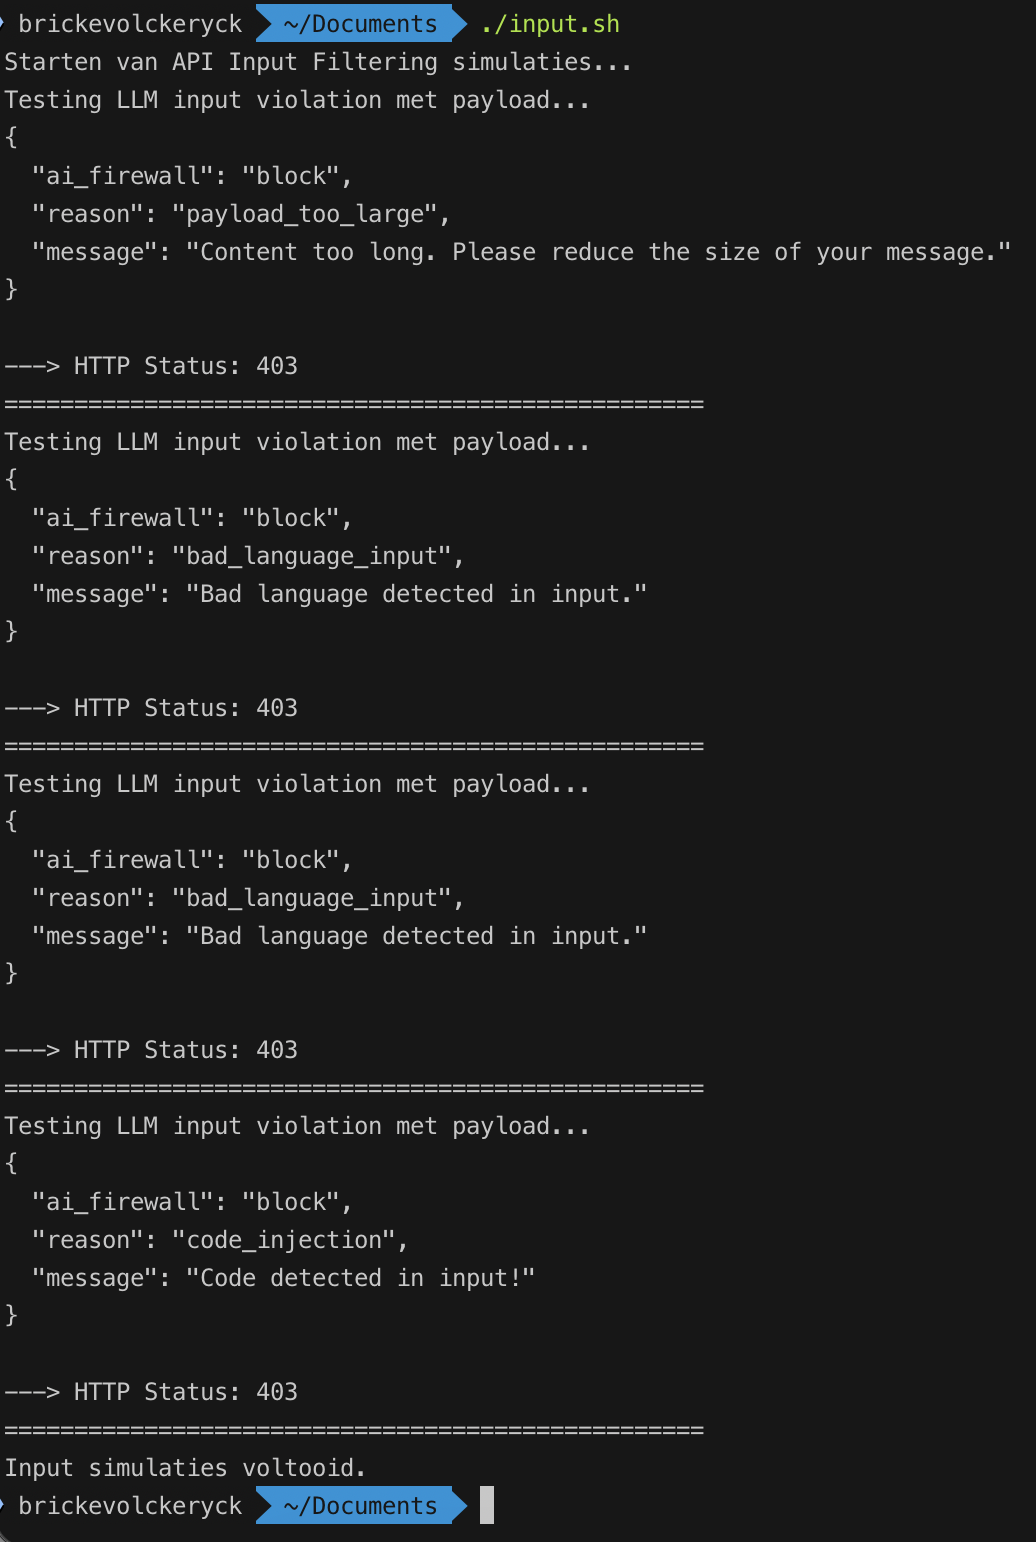
\includegraphics[width=0.5\textwidth]{img/input.png}
    \caption{Results of executing ./input.sh}
    \label{fig:input}
\end{figure}

Voor een gebruiker van de chatbot gaat dit er natuurlijk anders uit zien. Hiervoor heb ik in de index.html een stuk javascript toegevoegd dat het duidelijk maakt aan de gebruiker dat zijn prompt geblokkeerd is en waarom.

\begin{figure}[H]
    \centering
    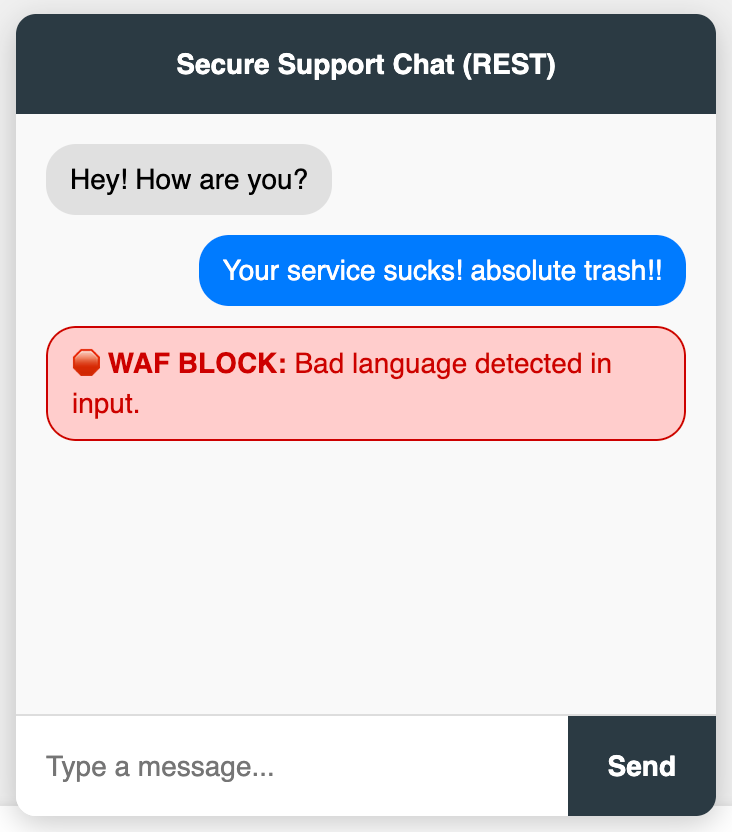
\includegraphics[width=0.5\textwidth]{img/wafblock.png}
    \caption{Screenshot of what a user would see}
    \label{fig:wafblock}
\end{figure}

\subsection{De Rol en Beperkingen van Output Filtering}

Waar de geautomatiseerde CLI-tests succesvol aantonen dat schadelijke input geblokkeerd wordt, hanteert Akamai eveneens beleidsregels voor Output Filtering (zoals "Toxic content on LLM output" en "Code detected on LLM output"). Het valideren van deze output-regels vereist echter een fundamenteel andere, minder automatiseerbare aanpak.\\

Output vormt in de kern pas een direct gevaar wanneer de onderliggende database of backend al blootgesteld is. Een chatbot zal uit zichzelf niet snel malafide code of ernstige PII genereren, tenzij deze data al in de aangesproken systemen zit (bijvoorbeeld door een eerdere Stored XSS-aanval via een onbeveiligd admin-paneel, of door foutieve brondata).\\

Wanneer een gebruiker de chatbot een legitieme vraag stelt, en de bot haalt vervolgens deze reeds 'vervuilde' data uit de database om als antwoord te dienen, dient de Output Filter van de Firewall for AI als een ultieme fail-safe. Het verbreekt de verbinding op het moment dat de geïnfecteerde respons de edge-server passeert. Omdat deze situatie sterk afhankelijk is van vooraf bestaande datacorruptie en complexe, meervoudige aanvalspatronen, is het simuleren van een output-blokkade sterk contextafhankelijk en uitdagend om in een simpel Bash-script te automatiseren. Dergelijke validaties zijn binnen deze Proof of Concept dan ook primair via gerichte, handmatige datamanipulatie-tests in de backend geverifieerd.

\section{Dashboards en Rapportage}

De effectiviteit van een gelaagde beveiligingsarchitectuur is sterk afhankelijk van de mate waarin incidenten inzichtelijk worden gemaakt voor beheerders. De integratie van Akamai en Dynatrace genereert een enorme hoeveelheid ruwe telemetrie- en netwerkdata. Om deze data om te zetten in bruikbare actionable insights, zijn op maat gemaakte dashboards geconfigureerd. Deze dashboards vormen de tastbare deliverables van de observability- en security-monitoring en bieden in één oogopslag inzicht in de gezondheid en veiligheid van de applicatie.

\subsection{Akamai Security-Dashboard}

Het Akamai Security Center dient als het primaire controlepaneel voor netwerk- en applicatiebeveiliging. Dit dashboard visualiseert alle interventies die door de Edge Firewall zijn uitgevoerd, met een specifieke nadruk op de recent geconfigureerde AI/LLM-regels.\\

Wanneer het script uit sectie 5.5 een malafide payload (zoals een Toxic Content of Code Injection prompt) verstuurt, genereert Akamai direct een Security Event. In het dashboard worden deze events geaggregeerd en geclassificeerd. Het toont niet alleen het totale volume aan geblokkeerde verzoeken, maar biedt ook gedetailleerde threat intelligence. Zo kan een beheerder per incident de herkomst (IP-adres en geolocatie), de getriggerde Firewall for AI-regel (bijv. "LLM input includes a non-allowed language") en de unieke Reference Error String inzien. Deze referentiecode correspondeert exact met de 403 Forbidden body die de aanvaller of frontend ontvangt, wat snelle correlatie en root-cause analysis bij false positives mogelijk maakt.\\

\begin{figure}[H]
    \centering
    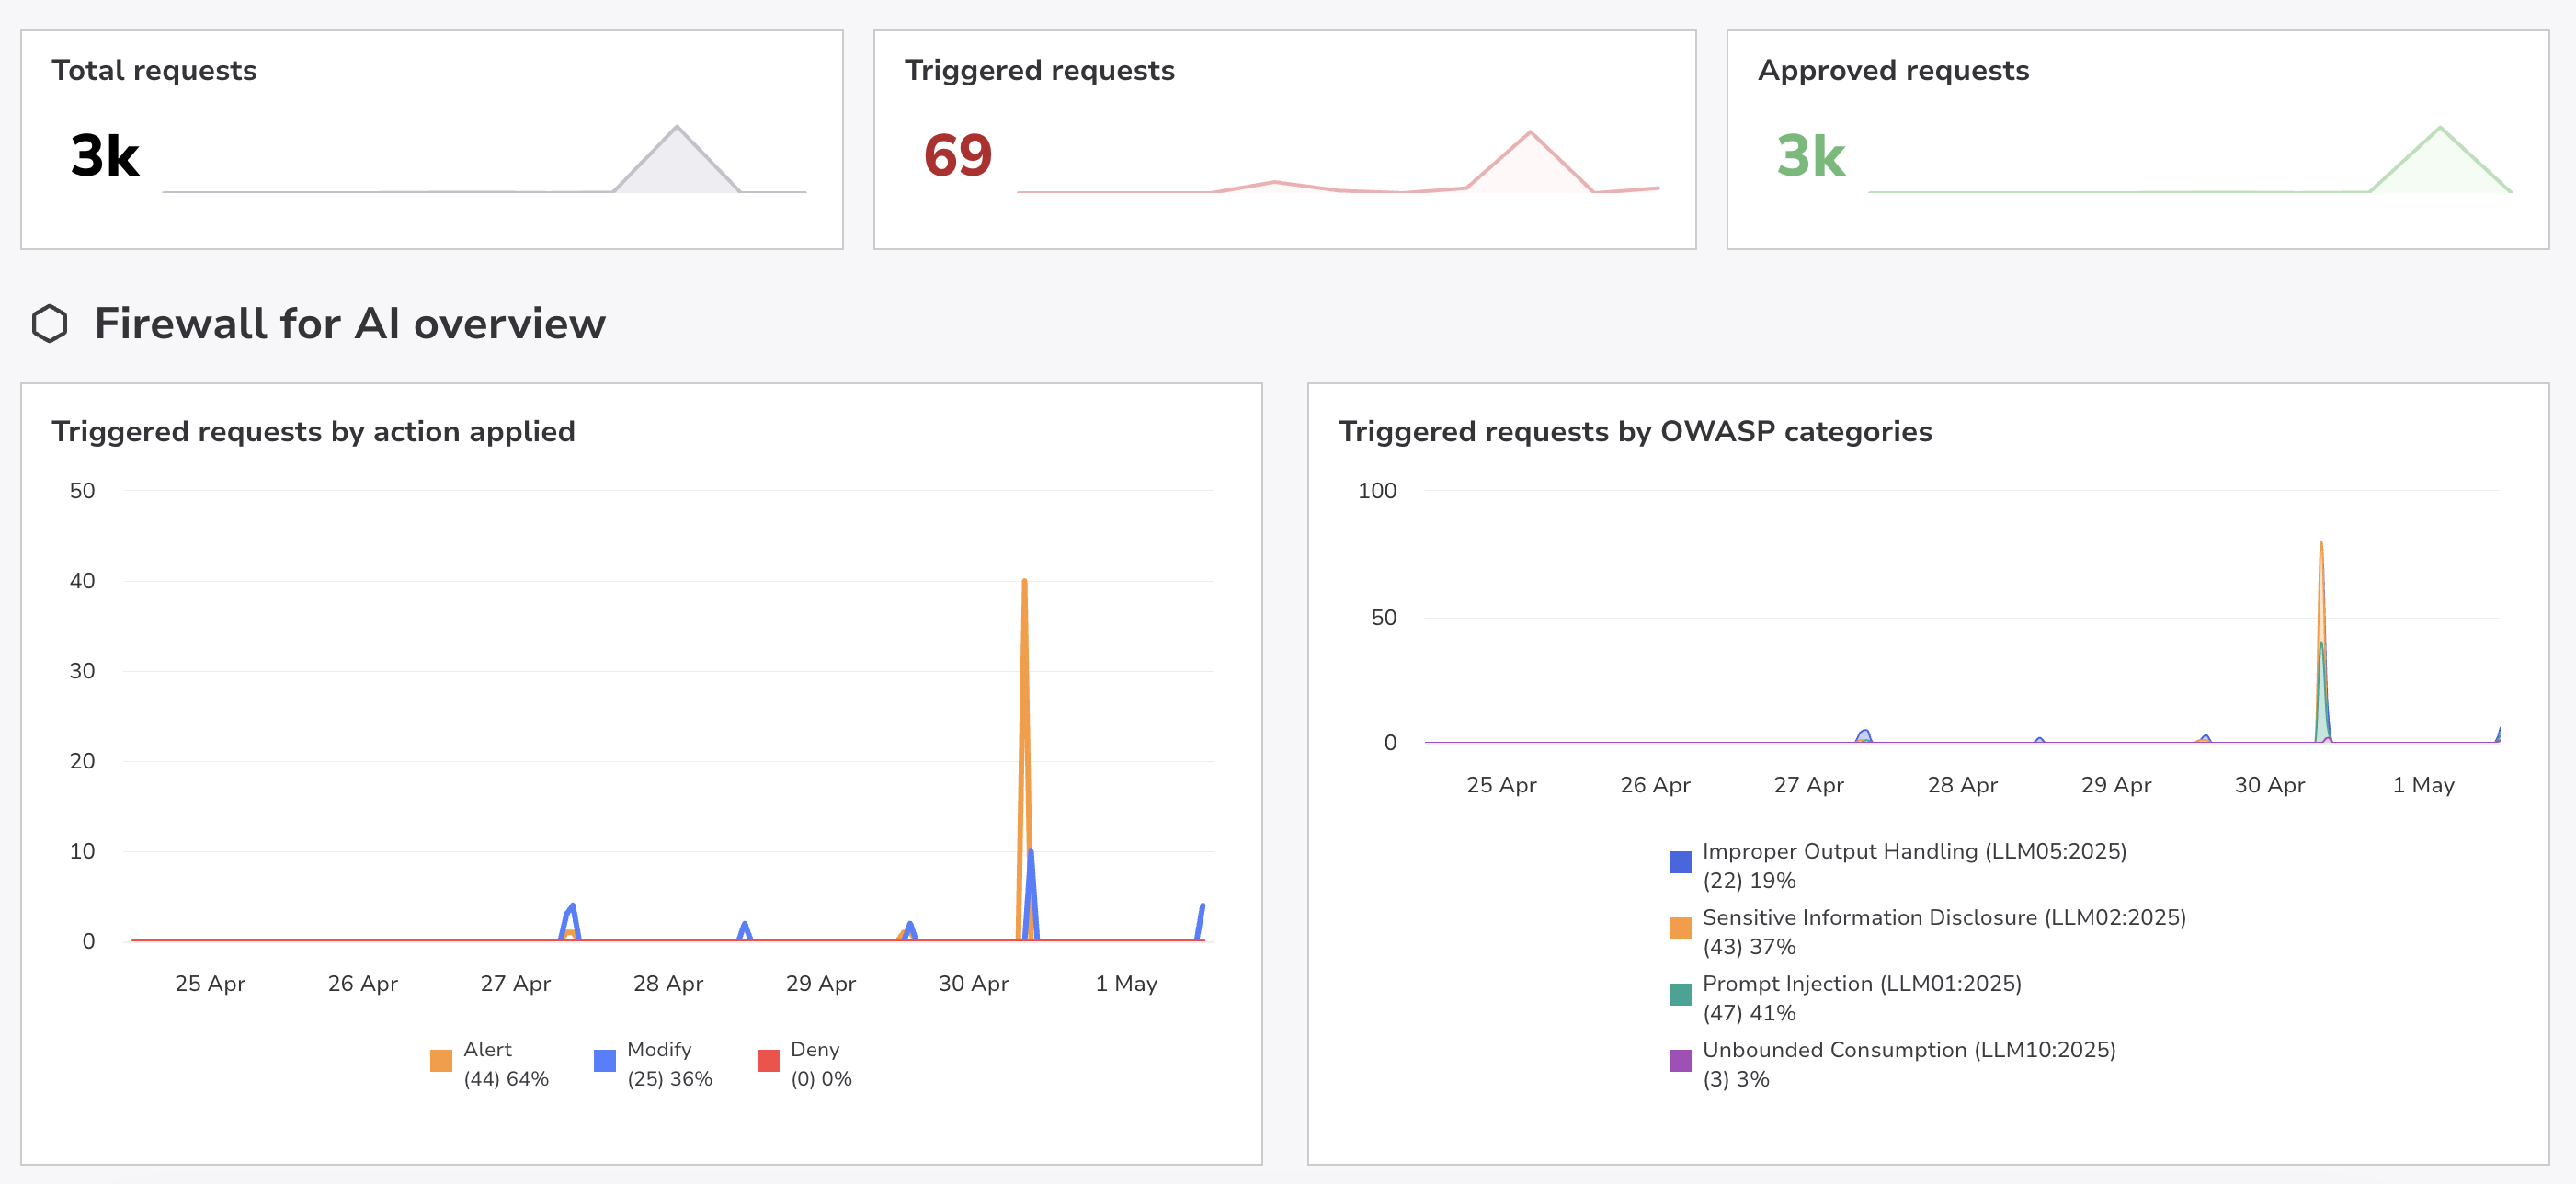
\includegraphics[width=0.75\textwidth]{img/akamaiDashboard.png}
    \caption{Firewall for AI dashboard van Akamai}
    \label{fig:akamaidash}
\end{figure}

\subsection{Dynatrace Conversatie- en Observability-Dashboard}
\textbf{TODO}

\section{GDPR Compliance en Privacy-by-Design}

Voor een applicatie die natural language verwerkt—zoals een digitale assistent—is gegevensbescherming een complexe uitdaging. Gebruikers kunnen in een vrij tekstveld onbewust, of uit onwetendheid, gevoelige persoonsgegevens (PII) invoeren, zoals wachtwoorden, rijksregisternummers of medische context. Om te voldoen aan de Algemene Verordening Gegevensbescherming (AVG/GDPR), is het principe van Privacy-by-Design vanaf de basis in de hybride architectuur verwerkt.

\subsection{Data Masking}
\textbf{TODO}

\subsection{Right to be Forgotten}
\textbf{TODO}